% Section 4: rectified flow head swap with FLUX.2-klein-4B.
% Numbers come from diffusion/faceswap_20_metrics_summary.csv and diffusion/REPORT.md.
% Figure inputs are relative to docs/report/.

\section{Rectified Flow Head Swap}

\subsection{Scope and hardware}
We wanted to swap a video face with one from a selfie. The run had to stay on one laptop with a 4 GB NVIDIA GPU and 8 GB of system RAM. We sent no data to a cloud service.

The output had to keep the source motion, expression, lighting and background. Only the head should change. The clip is 96 frames at 512x512 and lasts 3.2 seconds.

\subsection{How we measured}
Every number comes from one script run on the same 96 frames, and the results table reports it. Face change is how much the face region moves from one frame to the next. The unswapped footage sets the level to match, so a value far below it means the smoother removed real motion too. Consecutive identity is how similar a face is to the one before it, measured in a face recognition embedding, so higher is more stable. Identity to the portrait measures similarity to the reference portrait; the unswapped footage scores near zero because it is a different person. Hair noise is how much the hair region flickers, and lower is better; p95 marks the worst frames, the value 95 percent stay under.

\subsection{Pipeline overview}
The flow has four stages. Generation transfers the identity, restoration cleans each face with GFPGAN, smoothing removes the boil, and reassembly attaches the audio. Only the last stage writes a video file.

The boil is the flicker that comes from generating each frame on its own. Figure~\ref{fig:pipeline_overview} shows the chain in order, with the cost of each stage.

% Figure: pipeline overview of the face-reenactment flow (four stages).
% Facts and numbers come from diffusion/REPORT.md.
% Requires in the preamble: \usepackage{tikz} + \usetikzlibrary{arrows.meta}
\begin{figure}[t]
  \centering
  \begin{tikzpicture}[
    x=1cm, y=1cm,
    font=\small,
    block/.style={rectangle, rounded corners=2pt, draw=black!70, line width=0.5pt,
      fill=blue!10, align=center, inner sep=4pt, minimum height=9mm},
    inputblock/.style={rectangle, rounded corners=2pt, draw=black!70, line width=0.5pt,
      fill=green!12, align=center, inner sep=4pt, minimum height=9mm},
    stageblock/.style={rectangle, rounded corners=2pt, draw=black!70, line width=0.5pt,
      fill=orange!15, align=center, inner sep=4pt, minimum height=9mm},
    noteblock/.style={rectangle, rounded corners=2pt, draw=black!45, dashed,
      fill=red!8, align=left, inner sep=3pt, font=\scriptsize},
    flow/.style={->, >=Latex, line width=0.7pt, draw=black!75},
    arrowlab/.style={font=\scriptsize, fill=white, inner sep=1pt},
    cost/.style={draw=black!25, rounded corners=1pt, fill=gray!10, align=center,
      inner sep=3pt, font=\scriptsize, text width=2.6cm},
  ]

  % ---------------- inputs (left) ----------------
  \node[inputblock, inner xsep=2pt, text width=1.70cm, minimum height=1.46cm] (inP) at (0.96,1.90)
    {\textbf{Portrait}\\\textbf{256x256}\\[1pt]\scriptsize identity only};
  \node[inputblock, inner xsep=2pt, text width=2.10cm] (inB) at (1.16,-0.0806)
    {\textbf{Body frame}\\\textbf{512x512}\\[1pt]\scriptsize centre crop of
     the source video};
  \node[inputblock, inner xsep=2pt, text width=2.55cm] (inF) at (1.38,-2.20)
    {\textbf{Fixed prompt,}\\\textbf{409 characters}\\[1pt]\scriptsize names Picture 1\\and Picture 2};

  % ---------------- four stages (left to right) ----------------
  \node[stageblock, inner xsep=2pt, text width=2.81cm, minimum height=1.60cm] (S1) at (4.455,0)
    {\textbf{GENERATION}\\[1pt] makes the frames};
  \node[stageblock, inner xsep=2pt, text width=3.03cm, minimum height=1.60cm] (S2) at (7.735,0)
    {\textbf{RESTORATION}\\[1pt] cleans each face};
  \node[stageblock, inner xsep=2pt, text width=2.62cm, minimum height=1.60cm] (S3) at (10.920,0)
    {\textbf{SMOOTHING}\\[1pt] removes the boil};
  \node[stageblock, inner xsep=2pt, text width=2.80cm, minimum height=1.60cm] (S4) at (13.990,0)
    {\textbf{REASSEMBLY}\\[1pt] encodes and\\attaches the sound};

  % ---------------- input arrows into stage 1 ----------------
  \draw[flow] (inP.east) -- (S1.west |- 0,0.55);
  \draw[flow] (inB.east) -- (S1.west);
  \draw[flow] (inF.east) -- (S1.west |- 0,-0.55);

  % ---------------- data between the stages ----------------
  \draw[flow] (S1.east) -- (S2.west);
  \draw[flow] (S2.east) -- (S3.west);
  \draw[flow] (S3.east) -- (S4.west);
  \node[arrowlab] at (6.04,1.15) {96 raw frames};
  \node[arrowlab] at (9.43,1.15) {restored frames};
  \node[arrowlab] at (12.41,1.15) {smoothed frames};

  % ---------------- final output ----------------
  \node[inputblock, text width=3.12cm, minimum height=1.10cm] (out) at (13.75,2.05)
    {\textbf{512x512 clip, 3.203 s}};
  \draw[flow] (S4.north -| 13.75,0) -- (13.75,1.47);

  % ---------------- per-stage cost lines ----------------
  \node[cost, anchor=north] at (4.455,-0.95)
    {16.3 s per frame\\26.1 minutes in\\total};
  \node[cost, anchor=north] at (7.735,-0.95)
    {GFPGAN\\0.23 s per frame};
  \node[cost, anchor=north] at (10.920,-0.95)
    {optical flow\\strength 0.3\\0.036 s per frame};
  \node[cost, anchor=north] at (13.990,-0.95)
    {H.264, yuv420p, crf 18\\29.969 fps\\original audio muxed back};

  % ---------------- notes ----------------
  \node[noteblock, execute at begin node=\raggedright, text width=5.60cm, anchor=north west] at (3.30,-3.45)
    {\textbf{Safety gate:} a face detector counts faces before a frame is
     rendered. A frame with more than one face is refused. There is no bypass.};
  \node[noteblock, execute at begin node=\raggedright, text width=5.85cm, anchor=north west] at (9.35,-3.45)
    {Only the last stage writes a video file. Every earlier stage works on PNG frames.};

  % ---------------- legend ----------------
  \node[font=\scriptsize, anchor=north west] (leg) at (0.10,-3.45)
    {\begin{tabular}{@{}c@{\hspace{3pt}}l@{}}
       \tikz\fill[draw=black!70,line width=0.4pt,green!12] (0,0) rectangle (0.30,0.20); & input / output data\\
       \tikz\fill[draw=black!70,line width=0.4pt,blue!10]  (0,0) rectangle (0.30,0.20); & processing block\\
       \tikz\fill[draw=black!70,line width=0.4pt,orange!15](0,0) rectangle (0.30,0.20); & pipeline stage\\
       \tikz\fill[draw=black!45,line width=0.4pt,red!8]    (0,0) rectangle (0.30,0.20); & note / gate\\
     \end{tabular}};

  \end{tikzpicture}
  \caption{The four-stage pipeline: generation, restoration, smoothing and
    reassembly, with the cost measured for each stage.}
  \label{fig:pipeline_overview}
\end{figure}

\subsection{How a rectified flow model works}
A rectified flow model learns one job: connect a clean image and noise with a straight line. Training picks one random time per example and mixes the two ends at that time. The model predicts the direction that points from the noise end to the image end. The guess is compared with the true direction along the line, and the weights are then nudged.

At sampling time the same model starts from pure noise. Each Euler step moves the sample a small way along the predicted direction, and an image forms. The sampling code calls these steps denoising steps, because the sample becomes less noisy at each step. Figure~\ref{fig:diffusion_process} draws training and sampling side by side.

We did not train the base model; we used a released checkpoint. The released model is step distilled, so four steps are enough for it. We could not tell the difference between four steps and eight, and eight took twice the time.

% Figure: the two directions of the diffusion model.
% The forward direction is the training direction; the reverse direction is what the run uses.
% Facts come from the published model repository and model card.
% Requires in the preamble: \usepackage{tikz} + \usetikzlibrary{positioning,arrows.meta}
\begin{figure}[t]
  \centering
  \begin{tikzpicture}[
    x=1cm, y=1cm,
    font=\small,
    block/.style={rectangle, rounded corners=2pt, draw=black!70, line width=0.5pt,
      fill=blue!10, align=center, inner sep=4pt, minimum height=9mm},
    inputblock/.style={block, fill=green!12},
    stageblock/.style={block, fill=orange!15},
    noteblock/.style={rectangle, rounded corners=2pt, draw=black!45, dashed,
      fill=red!8, align=left, inner sep=3pt, font=\scriptsize},
    flow/.style={->, >=Latex, line width=0.7pt, draw=black!75},
    feed/.style={->, >=Latex, line width=0.7pt, draw=black!75, dashed},
    arrowlab/.style={font=\scriptsize, fill=white, inner sep=1pt},
  ]

  % ================= top half: how it was trained =================
  \node[anchor=west] (headT) at (0.15,10.35) {\textbf{How it was trained}};
  \node[font=\scriptsize, anchor=west, right=0.75cm of headT] (dirT) {the forward direction};
  \draw[flow] (dirT.east) -- ++(1.70,0);

  \node[inputblock, anchor=west, text width=1.75cm, minimum height=1.15cm] (clean) at (0.15,9.35)
    {clean\\image};
  \node[stageblock, text width=1.45cm, minimum height=1.15cm, right=0.45cm of clean] (add1)
    {add noise,\\[1pt]\scriptsize small};
  \node[stageblock, text width=1.45cm, minimum height=1.15cm, right=0.45cm of add1] (add2)
    {add noise,\\[1pt]\scriptsize more};
  \node[stageblock, text width=1.45cm, minimum height=1.15cm, right=0.45cm of add2] (add3)
    {add noise,\\[1pt]\scriptsize more};
  \node[inputblock, text width=1.70cm, minimum height=1.15cm, right=0.45cm of add3] (noiseA)
    {pure noise};
  \draw[flow] (clean) -- (add1);
  \draw[flow] (add1) -- (add2);
  \draw[flow] (add2) -- (add3);
  \draw[flow] (add3) -- (noiseA);

  % ---------------- the training loop under that chain ----------------
  \node[block, anchor=west, text width=3.20cm, minimum height=1.55cm] (lt1) at (0.15,7.75)
    {the network sees a noisy image and guesses the noise};
  \node[block, text width=3.20cm, minimum height=1.55cm, right=0.50cm of lt1] (lt2)
    {compare the guess with the noise that was really added};
  \node[block, text width=1.90cm, minimum height=1.55cm, right=0.50cm of lt2] (lt3)
    {nudge the weights};
  \draw[flow] (lt1) -- (lt2);
  \draw[flow] (lt2) -- (lt3);
  \draw[flow] (lt3.south) -- ++(0,-0.75) coordinate (retc) -- (retc -| lt1.south) -- (lt1.south);

  % ---------------- the one box that both halves use ----------------
  \path (lt1.center) -- (lt3.center) coordinate[midway] (loopmid);
  \coordinate (retmid) at (loopmid |- retc);
  \node[block, text width=3.40cm, minimum height=0.90cm] (net) at ([yshift=-1.00cm]retmid)
    {\textbf{the same network}};
  \draw[feed] (retmid) -- (net.north);

  % ================= bottom half: what we actually run =================
  \node[inputblock, anchor=west, text width=1.35cm, minimum height=1.15cm] (noiseB) at (0.15,3.65)
    {pure\\noise};
  \node[stageblock, text width=1.30cm, minimum height=1.15cm, right=0.45cm of noiseB] (st1)
    {denoise\\step};
  \node[stageblock, text width=1.30cm, minimum height=1.15cm, right=0.45cm of st1] (st2)
    {denoise\\step};
  \node[stageblock, text width=1.30cm, minimum height=1.15cm, right=0.45cm of st2] (st3)
    {denoise\\step};
  \node[stageblock, text width=1.30cm, minimum height=1.15cm, right=0.45cm of st3] (st4)
    {denoise\\step};
  \node[inputblock, text width=1.40cm, minimum height=1.15cm, right=0.45cm of st4] (latentB)
    {clean\\latent};
  \draw[flow] (noiseB) -- (st1);
  \draw[flow] (st1) -- (st2);
  \draw[flow] (st2) -- (st3);
  \draw[flow] (st3) -- (st4);
  \draw[flow] (st4) -- (latentB);

  % the same network drives every denoise step
  \coordinate (busY) at (0,4.40);
  \draw[feed] (net.south) -- (net.south |- busY);
  \draw[draw=black!75, line width=0.7pt, dashed] (st1.north |- busY) -- (st4.north |- busY);
  \foreach \s in {st1,st2,st3,st4}{\draw[feed] (\s.north |- busY) -- (\s.north);}

  \node[anchor=west] (headB) at (0.15,2.35) {\textbf{What we actually run}};
  \node[font=\scriptsize, anchor=west, right=0.75cm of headB] (dirB) {the reverse direction};
  \draw[flow] (dirB.east) -- ++(1.70,0);

  % ================= notes =================
  \node[noteblock, text width=3.55cm, anchor=north west] at (11.50,10.35)
    {Training needs a very large image set and many GPU hours. We did not train this model.
     We used a released checkpoint and trained only a small adapter on top of it.};
  \node[noteblock, text width=6.95cm, anchor=west] at (7.70,5.40)
    {The network only ever learns to remove noise. The reverse chain is what produces an image.};
  \node[noteblock, text width=7.20cm, anchor=north west] at (0.15,1.85)
    {The model is step distilled, so four steps are close to what a slow model would reach
     in dozens of steps.};
  \node[noteblock, text width=7.20cm, anchor=north west] at (7.65,1.85)
    {We never run the forward direction. It only exists so the network can learn.};

  \end{tikzpicture}
  \caption{The two directions of the diffusion model. The forward direction adds noise and is
    only used in training; the reverse direction removes noise and produces the image. Both
    directions use one and the same network.}
  \label{fig:diffusion_process}
\end{figure}

\subsection{The model and the LoRA adapter}
The model is a stack of transformer blocks (Figure~\ref{fig:architecture_lora}). A latent token of 128 channels is projected to width 3072. It passes through five double-stream blocks, then 20 single-stream blocks and a final layer. In the first part the text and image tokens stay apart, and they meet through joint attention.

Later the two streams are joined into one. The final layer projects back to 128 channels for the decoder.

The adapter is a small pair of matrices, A and B, trained beside each frozen weight. The adapter attaches inside the transformer blocks. It takes the attention projections and the feed-forward linears, and in the single-stream blocks the two fused linears. The block output adds a scaled product of A and B to the frozen term. Only A and B are trained, so the base weights never change. The adapter carries the head swap behaviour.

% Figure: the denoiser drawn as a stack of layers, and the LoRA adapter on one linear layer.
% Facts come from the published model repository and model card.
% Requires in the preamble: \usepackage{tikz} + \usetikzlibrary{positioning,arrows.meta},
%                            and amsmath for \frac in the adapter formula.
\begin{figure}[t]
  \centering
  \begin{tikzpicture}[
    x=1cm, y=1cm,
    font=\small,
    block/.style={rectangle, rounded corners=2pt, draw=black!70, line width=0.5pt,
      fill=blue!10, align=center, inner sep=4pt, minimum height=9mm},
    inputblock/.style={block, fill=green!12},
    stageblock/.style={block, fill=orange!15},
    noteblock/.style={rectangle, rounded corners=2pt, draw=black!45, dashed,
      fill=red!8, align=left, inner sep=3pt, font=\scriptsize},
    flow/.style={->, >=Latex, line width=0.7pt, draw=black!75},
    feed/.style={->, >=Latex, line width=0.7pt, draw=black!75, dashed},
    arrowlab/.style={font=\scriptsize, fill=white, inner sep=1pt},
  ]

  % ================= left part: the denoiser as a stack of layers =================
  \node[inputblock, anchor=north, text width=6.40cm, minimum height=0.90cm] (lat) at (6.54,10.55)
    {\textbf{latent token}, 128 channels};
  \node[block, text width=6.40cm, minimum height=0.90cm, below=0.32cm of lat] (proj)
    {\textbf{input projection} to width 3072};
  \node[block, text width=6.40cm, minimum height=1.15cm, below=0.32cm of proj] (tstep)
    {\textbf{timestep embedding}\\[1pt]\scriptsize sets scale and shift for every block};
  \node[block, text width=6.40cm, minimum height=1.15cm, below=0.32cm of tstep] (ds)
    {\textbf{5 double-stream blocks}\\[1pt]\scriptsize text and image tokens stay apart,
     joint attention};
  \node[block, text width=6.40cm, minimum height=0.90cm, below=0.32cm of ds] (cat)
    {\textbf{concatenate the two streams}};
  \node[block, text width=6.40cm, minimum height=1.15cm, below=0.32cm of cat] (ss)
    {\textbf{20 single-stream blocks}\\[1pt]\scriptsize one stream, joint attention};
  \node[block, text width=6.40cm, minimum height=1.15cm, below=0.32cm of ss] (fin)
    {\textbf{final layer}\\[1pt]\scriptsize adaptive layer norm, project to 128 channels};
  \node[inputblock, text width=6.40cm, minimum height=0.90cm, below=0.32cm of fin] (latout)
    {\textbf{latent}, to the decoder};
  \foreach \a/\b in {lat/proj, proj/tstep, tstep/ds, ds/cat, cat/ss, ss/fin, fin/latout}
    {\draw[flow] (\a.south) -- (\b.north);}

  % the text encoder enters through joint attention (dashed = conditioning path)
  \node[block, text width=2.10cm, left=0.70cm of cat] (enc)
    {\textbf{Qwen3-4B}\\[1pt]\scriptsize text encoder};
  \coordinate (txtcorner) at (enc.north |- ds.center);
  \draw[feed] (enc.north) -- (txtcorner) -- (ds.west);
  \path (txtcorner) -- (ds.west) coordinate[midway] (txtmid);
  \node[arrowlab, align=center, text width=1.70cm, anchor=south] at ([yshift=0.14cm]txtmid)
    {text tokens,\\width 7680};

  % the timestep embedding modulates every block (dashed = conditioning path)
  \draw[feed] (tstep.east) -- ++(0.35,0) coordinate (tbus);
  \draw[draw=black!75, line width=0.7pt, dashed] (tbus) -- (tbus |- fin.center);
  \foreach \s in {ds,ss,fin}{\draw[feed] (tbus |- \s.center) -- (\s.east);}

  % ================= right part: how the adapter attaches =================
  \node[inputblock, text width=2.40cm, minimum height=0.75cm] (layin) at (12.45,10.10)
    {layer input $x$};
  \node[block, text width=1.70cm, minimum height=2.35cm] (wgt) at (11.55,7.575)
    {\textbf{frozen weight $W$}};
  \node[block, text width=0.50cm, minimum height=0.90cm] (bA) at (13.35,8.30) {\textbf{A}};
  \node[block, text width=0.50cm, minimum height=0.90cm] (bB) at (13.35,6.85) {\textbf{B}};
  \draw[flow] (bA.south) -- (bB.north);

  \coordinate (br) at (12.45,9.30);
  \draw[draw=black!75, line width=0.7pt] (layin.south) -- (br);
  \draw[draw=black!75, line width=0.7pt] (br -| wgt.north) -- (br -| bA.north);
  \draw[flow] (br -| wgt.north) -- (wgt.north);
  \draw[flow] (br -| bA.north) -- (bA.north);

  \coordinate (mg) at (12.45,6.05);
  \draw[flow] (wgt.south) -- (mg -| wgt.south);
  \draw[flow] (bB.south) -- (mg -| bB.south);
  \draw[draw=black!75, line width=0.7pt] (mg -| wgt.south) -- (mg -| bB.south);
  \node[fill=white, inner sep=0.5pt] at (mg) {$+$};
  \node[inputblock, text width=1.85cm, minimum height=0.75cm] (layout) at (12.45,5.30)
    {output};
  \draw[flow] (mg) -- (layout.north);
  \node[font=\small] (formula) at (12.45,4.45) {$Wx + \frac{\alpha}{r}BAx$};

  \node[font=\scriptsize, align=left, text width=1.05cm, anchor=west] (abl) at (13.90,7.575)
    {rank $r$\\trained};

  % ================= notes =================
  \node[noteblock, text width=2.10cm, anchor=north west] at (0.12,3.40)
    {This layer stack is the published layout. We did not change it.};
  \node[noteblock, text width=4.40cm, anchor=north west] at (10.60,3.95)
    {Only A and B are trained. $W$ never changes, so the adapter is small and it can be
     removed again.};
  \node[noteblock, text width=4.40cm, anchor=north west] at (10.60,2.10)
    {The adapter has 100 modules. It teaches the base model the head swap task, so it changes
     what the model does, not how it looks.};

  \end{tikzpicture}
  \caption{The denoiser as a stack of layers. The text encoder and the timestep embedding enter
    as conditioning, and the adapter adds a small trained branch beside a frozen weight.}
  \label{fig:architecture_lora}
\end{figure}

\subsection{Generation}
Generation (Figure~\ref{fig:generation_architecture}) covers conditioning, sampling and decoding. A fixed prompt of 409 characters names Picture 1 as the body and Picture 2 as the head.

Qwen3-4B encodes the prompt once per session on the CPU, about 80 seconds, and its memory is then freed. Both pictures become VAE latents: the 512x512 body crop a 64x64x32 grid of about 1024 tokens, the 256x256 portrait about 256 tokens.

FLUX.2-klein-4B renders each frame in four sampling steps. Each step moves the latent along the direction the model predicts. The sampler calls the model once per step and feeds the result back. The text embeddings and the two image latents guide every step. A community-trained LoRA adapter of 80 adapted weights carries the head swap.

The same VAE decodes the final latent into pixels. Picture order is part of the adapter contract: the adapter's own documentation names Picture 1 the body and Picture 2 the head, and says not to reverse the images. A reversed order gives the wrong head.

The generator runs as a 4-bit GGUF file, and 256 pixels is the largest reference that fits. A detector refuses a frame with more than one face, and the gate has no bypass.

The output is 96 frames from 5.8 to 9.0 seconds of the source, all with one fixed seed. Each frame took 16.3 seconds, so the stage used 26.1 minutes.

% Figure: architecture of the generation stage (conditioning, denoising, decoding).
% Facts and numbers come from diffusion/REPORT.md.
% Requires in the preamble: \usepackage{tikz} + \usetikzlibrary{arrows.meta}
\begin{figure}[t]
  \centering
  \begin{tikzpicture}[
    x=1cm, y=1cm,
    font=\small,
    block/.style={rectangle, rounded corners=2pt, draw=black!70, line width=0.5pt,
      fill=blue!10, align=center, inner sep=4pt, minimum height=9mm},
    inputblock/.style={rectangle, rounded corners=2pt, draw=black!70, line width=0.5pt,
      fill=green!12, align=center, inner sep=4pt, minimum height=9mm},
    stageblock/.style={rectangle, rounded corners=2pt, draw=black!70, line width=0.5pt,
      fill=orange!15, align=center, inner sep=4pt, minimum height=9mm},
    noteblock/.style={rectangle, rounded corners=2pt, draw=black!45, dashed,
      fill=red!8, align=left, inner sep=3pt, font=\scriptsize},
    flow/.style={->, >=Latex, line width=0.7pt, draw=black!75},
    bundle/.style={->, >=Latex, line width=1.2pt, draw=black!75},
    feed/.style={line width=0.7pt, draw=black!75},
    arrowlab/.style={font=\scriptsize, fill=white, inner sep=1pt},
  ]

  % ---------------- conditioning (top) ----------------
  \node[inputblock, text width=2.55cm] (prompt) at (1.42,4.10)
    {\textbf{Fixed prompt,}\\\textbf{409 characters}\\[1pt]\scriptsize names Picture 1
     and Picture 2};
  \node[block, text width=4.45cm] (enc) at (5.60,4.10)
    {\textbf{Qwen3-4B text encoder}\\[1pt]\scriptsize CPU, 4 bit, about 80 s once per
     session, then its memory is freed};
  \node[block, text width=2.95cm] (emb) at (9.99,4.10) {\textbf{text embeddings}};
  \draw[flow] (prompt.east) -- (enc.west);
  \draw[flow] (enc.east) -- (emb.west);

  % ---------------- denoising chain (middle) ----------------
  \node[block, text width=4.45cm] (flux) at (2.37,2.10)
    {\textbf{FLUX.2-klein-4B}\\[1pt]\scriptsize 4 bit GGUF};
  \node[block, text width=5.70cm] (steps) at (8.19,2.10)
    {\textbf{4 denoising steps}\\[1pt]\scriptsize guided at every step};
  \node[block, text width=1.30cm] (dec) at (12.36,2.10) {\textbf{VAE}\\\textbf{decode}};
  \node[inputblock, text width=1.60cm] (frame) at (14.40,2.10)
    {\textbf{512x512}\\\textbf{frame}};
  \node[block, text width=2.60cm] (lora) at (1.74,0.35)
    {\textbf{LoRA adapter}\\[1pt]\scriptsize 100 modules};
  \draw[flow] (lora.north) -- (flux.south);
  \draw[flow] (flux.east) -- (steps.west);
  \draw[flow] (steps.east) -- (dec.west);
  \draw[flow] (dec.east) -- (frame.west);

  % ---------------- image branches (lower left) ----------------
  \node[inputblock, text width=2.10cm] (bodyf) at (1.19,-2.40)
    {\textbf{Body frame}\\\textbf{512x512}\\[1pt]\scriptsize centre crop of
     the source video};
  \node[block, text width=1.30cm] (vaeA) at (3.57,-2.40) {\textbf{VAE}\\\textbf{encode}};
  \node[block, text width=2.40cm] (latA) at (6.10,-2.40)
    {\textbf{64x64x32 latent}\\[1pt]\scriptsize about 1024 tokens};
  \draw[flow] (bodyf.east) -- (vaeA.west);
  \draw[flow] (vaeA.east) -- (latA.west);

  \node[inputblock, text width=1.70cm] (port) at (0.99,-4.40)
    {\textbf{Portrait}\\\textbf{256x256}\\[1pt]\scriptsize identity only};
  \node[block, text width=1.30cm] (vaeB) at (3.57,-4.40) {\textbf{VAE}\\\textbf{encode}};
  \node[block, text width=2.60cm] (latB) at (6.20,-4.40)
    {\textbf{about 256 tokens}\\[1pt]\scriptsize identity only};
  \draw[flow] (port.east) -- (vaeB.west);
  \draw[flow] (vaeB.east) -- (latB.west);

  % ---------------- conditioning into the denoising steps ----------------
  \draw[flow] (emb.south -| 10.10,0) -- (10.10,2.66);
  \draw[feed] (latA.east) -- (8.40,-2.40) -- (8.40,0.90) -- (8.95,0.90);
  \draw[feed] (latB.east) -- (9.40,-4.40) -- (9.40,0.90) -- (8.95,0.90);
  \draw[bundle] (8.95,0.90) -- (8.95,1.60);
  \node[font=\scriptsize, anchor=east, fill=white, inner sep=1pt] at (8.15,0.88) {2 image latents};

  % ---------------- notes ----------------
  \node[noteblock, text width=4.50cm, anchor=north west] at (3.50,0.60)
    {The LoRA changes 99.5 percent of the pixels against the unadapted model, so it
     changes the task, not the style.};
  \node[noteblock, text width=5.30cm, anchor=north west] at (9.80,1.13)
    {Four steps are enough. The base model is step distilled. Eight steps looked
     the same and took twice the time.};
  \node[noteblock, text width=5.30cm, anchor=north west] at (9.80,-0.27)
    {The order of the two pictures is part of the contract. Reversing them gives a
     plausible image with the wrong head.};
  \node[noteblock, text width=5.30cm, anchor=north west] at (9.80,-4.00)
    {A 512 pixel reference does not fit in the remaining memory. 256 pixels is the
     measured maximum.};

  % ---------------- legend ----------------
  \node[font=\scriptsize, anchor=north west] (leg) at (9.90,-2.30)
    {\begin{tabular}{@{}c@{\hspace{3pt}}l@{}}
       \tikz\fill[draw=black!70,line width=0.4pt,green!12] (0,0) rectangle (0.30,0.20); & input image\\
       \tikz\fill[draw=black!70,line width=0.4pt,blue!10]  (0,0) rectangle (0.30,0.20); & model block\\
       \tikz\fill[draw=black!45,line width=0.4pt,red!8]    (0,0) rectangle (0.30,0.20); & note\\
     \end{tabular}};

  \end{tikzpicture}
  \caption{Inside the generation stage: text conditioning, the image latents, the
    denoiser with its LoRA adapter, and the four denoising steps.}
  \label{fig:generation_architecture}
\end{figure}

\subsubsection{Adapter version comparison}
The recorded clip uses adapter v1 throughout. A newer adapter, v1.1, was released during the work, and we tested two prompt variants, A and B. Table~\ref{tab:adapters} compares the two versions.

v1.1 ran, but it went far past the memory of the card, which is why it slowed down so much. The v1.1 adapter has rank 512 against the 128 of v1, so it is four times larger. That is why it went past the card and slowed down. The extra time was not worth it for us.

We judged the look by eye and preferred v1, so the clip kept the v1 output. No metric script was run on v1.1, so every other number here comes from v1. The grids in Figure~\ref{fig:lora_compare} are the only evidence.

\begin{table}[tb]
  \centering
  \footnotesize
  \begin{tabular}{@{}l l l@{}}
    \toprule
    & v1 (recorded) & v1.1 (new) \\
    \midrule
    Adapter rank & 128 & 512 \\
    Seconds per frame & 16.34 & about 199, twelve times slower \\
    Peak VRAM allocated & 3.60 GiB & 4.68 GiB, past the 4.0 GiB of the card \\
    Peak system RAM & 5.48 GiB & 5.50 GiB \\
    Cost for 96 frames & 26 minutes & about 5.3 hours \\
    \bottomrule
  \end{tabular}
  \caption{Adapter v1 against v1.1 on the same machine; only v1 was measured with the metric script.}
  \label{tab:adapters}
\end{table}

\begin{figure}[t]
  \centering
  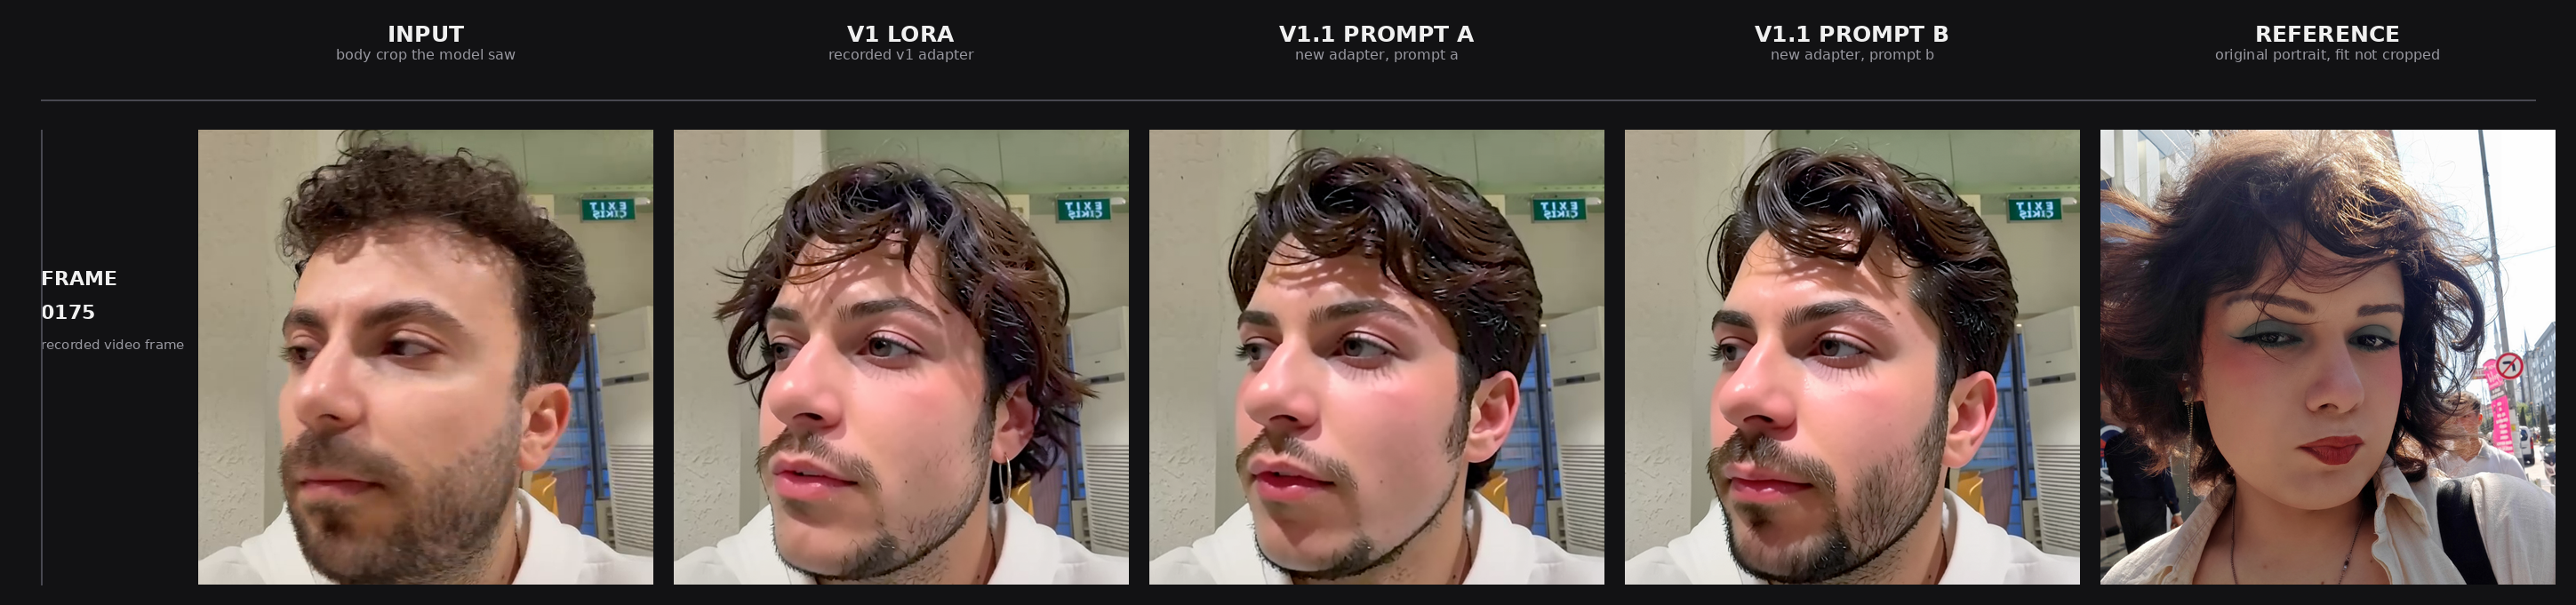
\includegraphics[width=\linewidth]{figures/faceswap_lora_compare_grid_0175.png}\\[3pt]
  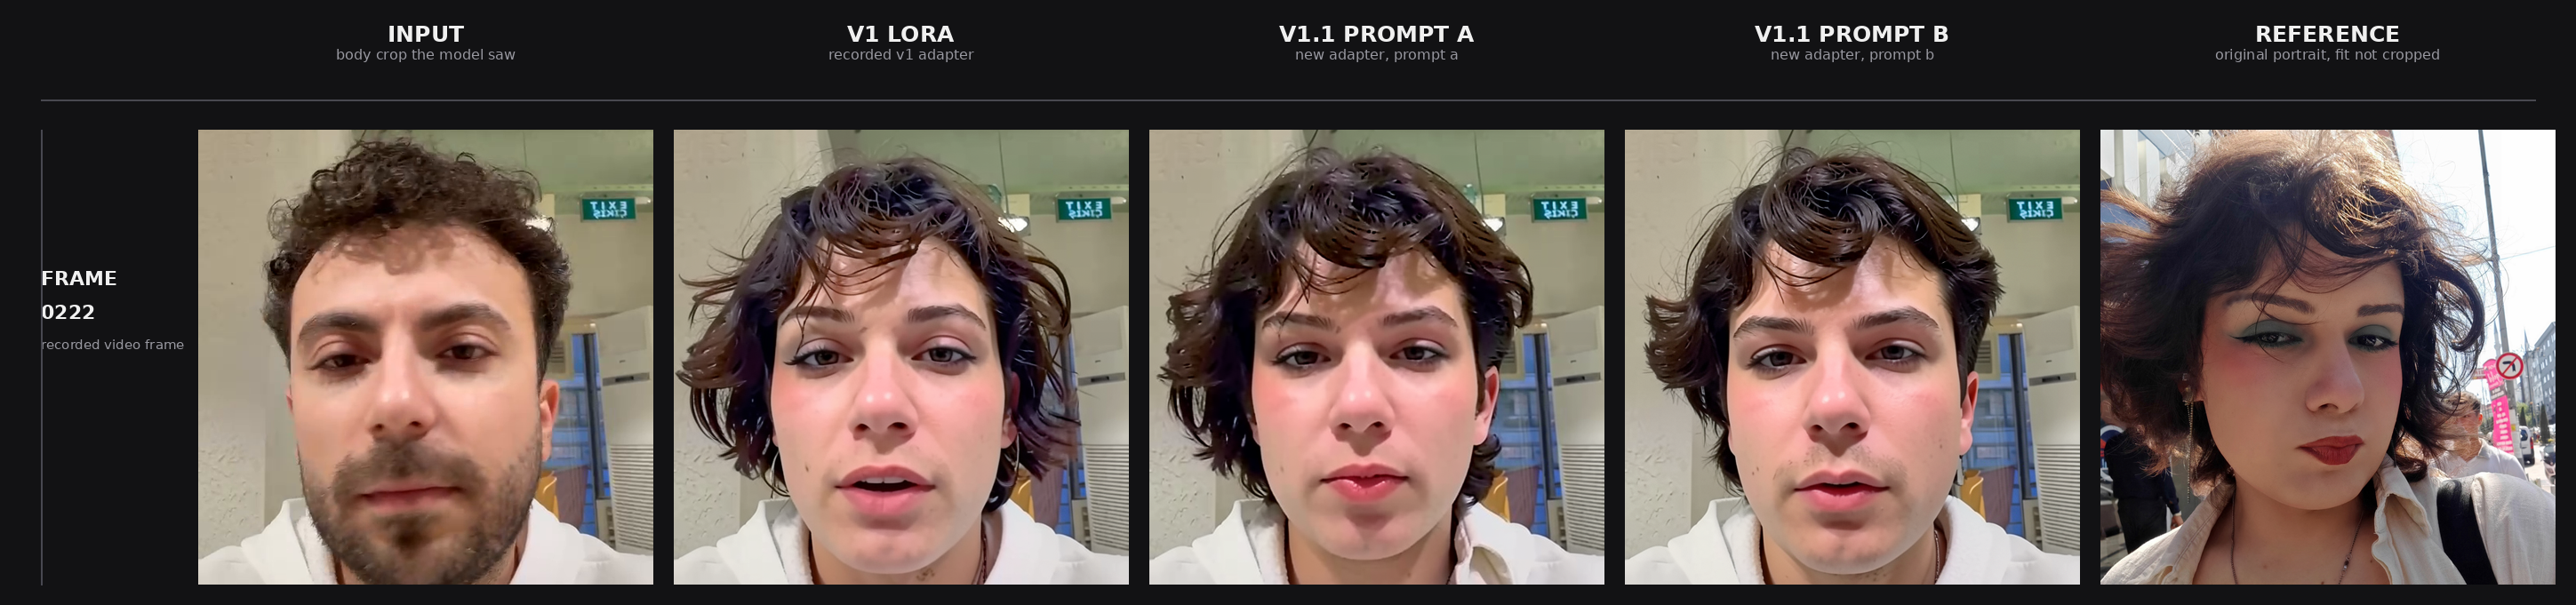
\includegraphics[width=\linewidth]{figures/faceswap_lora_compare_grid_0222.png}\\[3pt]
  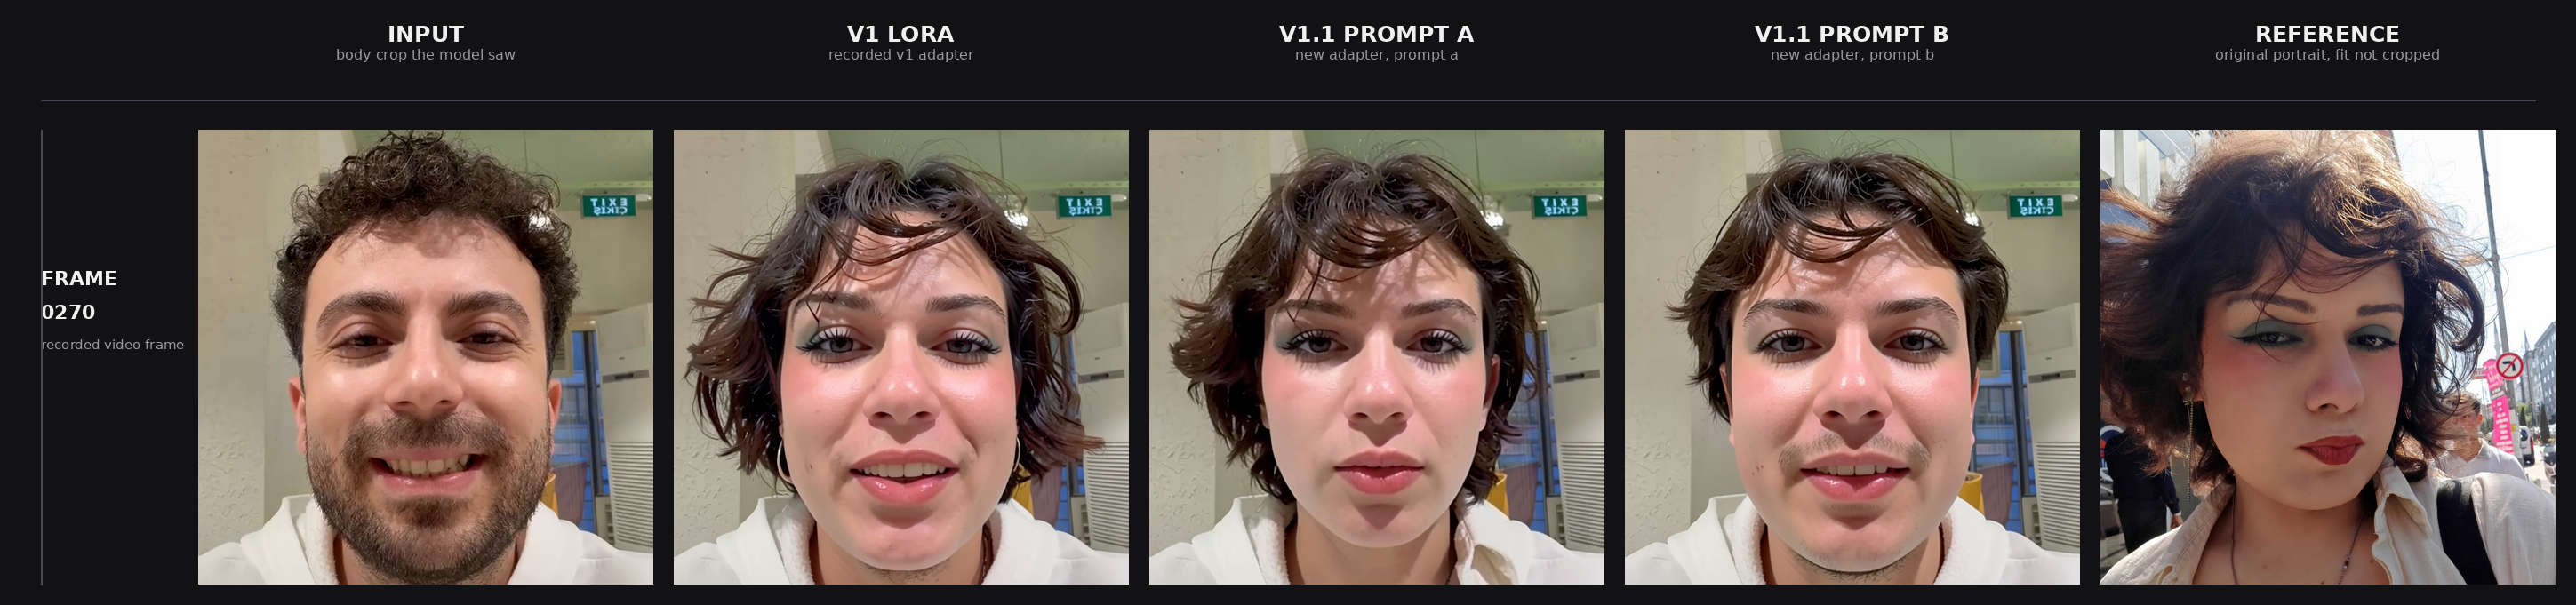
\includegraphics[width=\linewidth]{figures/faceswap_lora_compare_grid_0270.png}
  \caption{Each row is one source frame, the frame number printed inside. The five
  columns run from the input body crop through the v1 adapter, v1.1 with prompt A,
  v1.1 with prompt B, to the reference portrait; only the adapter version and the
  prompt variant change.}
  \label{fig:lora_compare}
\end{figure}

\subsection{Face restoration}
GFPGAN v1.4 cleans every frame (Figure~\ref{fig:restoration}). It detects and aligns the face, runs a restoration network, and composites the crop back. The weights are official, but we built the network in project code because the published wrappers do not import.

The stage costs 0.23 seconds per frame. The frames looked cleaner to us, and the mean face change came down, though the tail improved less.

Hair noise fell slightly, a small gain on its own. The fidelity weight does nothing, because the official inference path passes no weight argument. Restoration cannot remove flicker, because it sees one frame at a time.

% Figure: the face restoration stage (detect, align, restore, composite).
% Facts come from diffusion/REPORT.md, section 4.
% Requires in the preamble: \usepackage{tikz} + \usetikzlibrary{positioning,arrows.meta}
\begin{figure}[t]
  \centering
  \begin{tikzpicture}[
    x=1cm, y=1cm,
    font=\small,
    block/.style={rectangle, rounded corners=2pt, draw=black!70, line width=0.5pt,
      fill=blue!10, align=center, inner sep=4pt, minimum height=9mm},
    inputblock/.style={block, fill=green!12},
    stageblock/.style={block, fill=orange!15},
    noteblock/.style={rectangle, rounded corners=2pt, draw=black!45, dashed,
      fill=red!8, align=left, inner sep=3pt, font=\scriptsize},
    flow/.style={->, >=Latex, line width=0.7pt, draw=black!75},
    arrowlab/.style={font=\scriptsize, fill=white, inner sep=1pt},
  ]

  % ---------------- main row: frame in, detect and align, restore, composite, frame out
  \node[inputblock, text width=1.70cm] (raw) at (1.10,0)
    {raw frame\\[2pt]{\scriptsize as generated}};
  \node[stageblock, text width=2.30cm] (det) at (3.95,0)
    {detect and\\align the face\\[2pt]{\scriptsize a crop is taken}};

  % the restoration network: one container with a stack of three inner blocks
  \node[stageblock, minimum width=3.60cm, minimum height=4.90cm] (net) at (7.55,0) {};
  \node[anchor=north, inner sep=1pt] (nett) at ([yshift=-4pt]net.north)
    {\textbf{restoration network}};
  \node[anchor=north, inner sep=1pt, font=\scriptsize, text width=3.30cm, align=center]
    (nets) at ([yshift=-2pt]nett.south)
    {GFPGAN v1.4, trained to map degraded faces onto clean ones};
  \node[block, text width=2.60cm, minimum height=6mm] (enc) at (7.55,0.10) {encoder};
  \node[block, text width=2.60cm, minimum height=6mm] (dbl) at (7.55,-0.80) {detail blocks};
  \node[block, text width=2.60cm, minimum height=6mm] (dec) at (7.55,-1.70) {decoder};
  \draw[flow] (enc.south) -- (dbl.north);
  \draw[flow] (dbl.south) -- (dec.north);

  \node[stageblock, text width=2.30cm] (comp) at (11.15,0)
    {composite the\\crop back\\[2pt]{\scriptsize into the frame}};
  \node[inputblock, text width=1.75cm] (res) at (14.05,0)
    {restored\\frame};

  \draw[flow] (raw) -- (det);
  \draw[flow] (det) -- (net);
  \draw[flow] (net) -- (comp);
  \draw[flow] (comp) -- (res);

  % ---------------- notes ----------------
  \node[noteblock, execute at begin node=\raggedright, text width=7.00cm, anchor=north west] at (0.11,-2.70)
    {The weights are the official release. The network was rebuilt in project code
     because the published wrappers do not import.};
  \node[noteblock, execute at begin node=\raggedright, text width=7.50cm, anchor=north west] at (7.45,-2.70)
    {The fidelity weight does nothing. The official inference path passes no weight
     argument.};
  \node[noteblock, execute at begin node=\raggedright, text width=5.50cm, anchor=north west] at (9.60,2.20)
    {Restoration sees one frame at a time, so it cannot remove flicker.};

  \end{tikzpicture}
  \caption{The face restoration stage. Each raw frame is taken on its own: the face is
    detected and aligned, a crop runs through the restoration network, and the restored
    crop is composited back into the frame.}
  \label{fig:restoration}
\end{figure}

\subsection{Temporal smoothing}
The smoothing stage compares frames with each other and removes the boil (Figure~\ref{fig:smoothing}). The per-pixel deflicker averages each pixel with its temporal neighbours, and it is too strong. It costs 0.007 seconds per frame.

The deflicker pushes the face change below the unswapped level, so it removes real motion as well as the boil. Optical flow estimates the dense motion between neighbouring frames and warps them onto the current one. Because it follows the same surface point across time, a moving head does not smear. It costs 0.036 seconds per frame.

The control fixes the real motion level at 6.66, and the distance column is the face change minus that level. At strength 0.3 the chained pass comes close enough to the control, and the raw pass stays above it. A stronger setting sits below the control, which is over-smoothing.

The recommended output is the chained set at strength 0.3. It beats the flow-only variant on face change, on the tail and on hair noise. Only consecutive identity is slightly lower. The deflicker reaches its low face change only by destroying motion, so we kept flow.

\begin{table}[tb]
  \centering
  \footnotesize
  \setlength{\tabcolsep}{4pt}
  \begin{tabular}{@{}l r r r r r r@{}}
    \toprule
    \begin{tabular}[c]{@{}l@{}}Frames\\smoothed\end{tabular} & Strength &
    \begin{tabular}[c]{@{}r@{}}Face\\change\end{tabular} &
    \begin{tabular}[c]{@{}r@{}}Distance from\\the control\end{tabular} & p95 &
    \begin{tabular}[c]{@{}r@{}}Consecutive\\identity\end{tabular} &
    \begin{tabular}[c]{@{}r@{}}Hair\\noise\end{tabular} \\
    \midrule
    Raw & 0.3 & 6.9599 & +0.3034 & 16.2944 & 0.9330 & 32.2358 \\
    Raw & 0.6 & 6.6663 & +0.0098 & 15.6581 & 0.9391 & 32.0603 \\
    Restored, then flow & 0.3 & 6.6303 & -0.0262 & 15.2802 & 0.9377 & 31.7306 \\
    Restored, then flow & 0.6 & 6.3071 & -0.3494 & 14.7575 & 0.9431 & 31.5448 \\
    \bottomrule
  \end{tabular}
  \caption{The smoothing sweep: two frame sets at two strengths, all measured on the same 96 frames.}
  \label{tab:smooth}
\end{table}

% Figure: the temporal smoothing stage (optical flow between neighbouring frames).
% Facts come from diffusion/REPORT.md, section 5.
% Requires in the preamble: \usepackage{tikz} + \usetikzlibrary{positioning,arrows.meta}
\begin{figure}[t]
  \centering
  \begin{tikzpicture}[
    x=1cm, y=1cm,
    font=\small,
    block/.style={rectangle, rounded corners=2pt, draw=black!70, line width=0.5pt,
      fill=blue!10, align=center, inner sep=4pt, minimum height=9mm},
    inputblock/.style={block, fill=green!12},
    stageblock/.style={block, fill=orange!15},
    noteblock/.style={rectangle, rounded corners=2pt, draw=black!45, dashed,
      fill=red!8, align=left, inner sep=3pt, font=\scriptsize},
    flow/.style={->, >=Latex, line width=0.7pt, draw=black!75},
    arrowlab/.style={font=\scriptsize, fill=white, inner sep=1pt},
  ]

  % ---------------- three stacked input frames ----------------
  \node[inputblock, text width=1.35cm] (f0) at (1.15,2.05) {frame t-1};
  \node[inputblock, text width=1.35cm] (f1) at (1.15,0.00) {frame t};
  \node[inputblock, text width=1.35cm] (f2) at (1.15,-2.05) {frame t+1};

  % the window of frames enters the stage on one line
  \draw[draw=black!75, line width=0.7pt] (f0.east) -- (2.35,2.05);
  \draw[draw=black!75, line width=0.7pt] (f1.east) -- (2.35,0.00);
  \draw[draw=black!75, line width=0.7pt] (f2.east) -- (2.35,-2.05);
  \draw[draw=black!75, line width=0.7pt] (2.35,-2.05) -- (2.35,2.05);

  % ---------------- main row ----------------
  \node[stageblock, text width=3.10cm] (est) at (4.45,0)
    {estimate the\\dense motion\\[2pt]{\scriptsize flow between frame t\\and each neighbour}};
  \node[stageblock, text width=3.20cm] (warp) at (8.85,0)
    {warp both\\neighbours onto\\frame t\\[2pt]{\scriptsize the same surface point\\across time}};
  \node[stageblock, text width=1.60cm] (blend) at (12.00,0)
    {blend\\[2pt]{\scriptsize with frame t}};
  \node[inputblock, text width=1.70cm] (out) at (14.35,0)
    {smoothed\\frame t};

  \draw[flow] (2.35,0) -- (est.west);
  \draw[flow] (est.east) -- (warp.west);
  \node[arrowlab, anchor=south] at (6.62,0.20) {motion};
  \draw[flow] (warp.east) -- (blend.west);
  \draw[flow] (blend.east) -- (out.west);

  % the two neighbours also reach the warp
  \draw[draw=black!75, line width=0.7pt] (2.35,2.05) -- (2.35,2.95);
  \draw[flow] (2.35,2.95) -- (8.85,2.95) -- (warp.north);
  \node[arrowlab] at (5.30,2.95) {neighbour frames};

  % ---------------- strength input to the blend ----------------
  \node[block, text width=1.90cm] (str) at (12.00,-1.75) {strength 0.3};
  \draw[flow] (str.north) -- (blend.south);

  % ---------------- notes ----------------
  \node[noteblock, text width=6.90cm, anchor=north west] at (0.34,-2.95)
    {A per-pixel deflicker is cheaper. It averages each pixel with its temporal
     neighbours, and it removes real motion as well as the boil.};
  \node[noteblock, text width=7.20cm, anchor=north west] at (7.90,-2.75)
    {At strength 0.3 the result matches the motion level of the unswapped footage.
     At 0.6 the pass sits below it, which is over-smoothing.};

  \end{tikzpicture}
  \caption{The temporal smoothing stage. Each frame is compared with its two
    neighbours: the dense motion is estimated, the neighbours are warped onto frame t
    and the three are blended at strength 0.3.}
  \label{fig:smoothing}
\end{figure}

\subsection{Reassembly}
The encoder turns a frame set into a playable clip (Figure~\ref{fig:reassembly}). It writes H.264 at 29.969 fps, muxes the original audio back, and trims both streams. Its output is a 512x512 clip of 3.203 seconds.

The encode adds nothing to the pixels. In the raw swapped set the face boils, and the results table holds the values.

% Figure: the reassembly stage (encode the frames, mux the source audio back).
% Facts come from rectified_flow/final_report/REPORT.md, section 6.
% Requires in the preamble: \usepackage{tikz} + \usetikzlibrary{positioning,arrows.meta}
\begin{figure}[t]
  \centering
  \begin{tikzpicture}[
    x=1cm, y=1cm,
    font=\small,
    block/.style={rectangle, rounded corners=2pt, draw=black!70, line width=0.5pt,
      fill=blue!10, align=center, inner sep=4pt, minimum height=9mm},
    inputblock/.style={block, fill=green!12},
    stageblock/.style={block, fill=orange!15},
    noteblock/.style={rectangle, rounded corners=2pt, draw=black!45, dashed,
      fill=red!8, align=left, inner sep=3pt, font=\scriptsize},
    flow/.style={->, >=Latex, line width=0.7pt, draw=black!75},
    arrowlab/.style={font=\scriptsize, fill=white, inner sep=1pt},
  ]

  % ---------------- the two inputs ----------------
  \node[inputblock, text width=2.05cm] (vid) at (1.70,0.85) {smoothed frames};
  \node[inputblock, text width=2.05cm] (aud) at (1.70,-0.85) {source audio};

  % ---------------- main row ----------------
  \node[stageblock, text width=2.75cm] (enc) at (5.55,0.85)
    {encode H.264\\[2pt]{\scriptsize 29.969 fps, yuv420p,\\crf 18}};
  \node[stageblock, text width=3.30cm] (mux) at (10.35,0.85)
    {mux the audio back\\[2pt]{\scriptsize both streams are trimmed\\to the same length}};
  \node[inputblock, text width=2.25cm] (out) at (14.15,0.85)
    {final clip\\[2pt]{\scriptsize 512x512, 3.2 seconds}};

  \draw[flow] (vid.east) -- (enc.west);
  \draw[flow] (enc.east) -- (mux.west);
  \node[arrowlab] at (7.81,0.85) {video};
  \draw[flow] (mux.east) -- (out.west);

  % ---------------- the audio path, around the encoder ----------------
  \draw[flow] (aud.east) -- (10.35,-0.85) -- (mux.south);
  \node[arrowlab] at (5.60,-0.85) {audio};

  % ---------------- notes ----------------
  \node[noteblock, text width=7.10cm, anchor=north west] at (0.54,-2.20)
    {The encode is lossy: it changes pixels slightly, but it cannot alter the face
     motion.};
  \node[noteblock, text width=7.30cm, anchor=north west] at (8.10,2.60)
    {The same script is the last stage of the whole flow, so the final video is a
     later run of this encoder.};

  \end{tikzpicture}
  \caption{The reassembly stage. The smoothed frames are encoded as H.264 at the source
    rate and the original audio is muxed back; both streams are trimmed to the same
    length.}
  \label{fig:reassembly}
\end{figure}

\subsection{Results}
All numbers come from one script on the same 96 frames. Lower hair noise is better, and higher identity values are better. Face change should sit near the control level, because a value below it means the smoother removed real motion. The control row is the unswapped source footage.

\begin{table}[tb]
  \centering
  \footnotesize
  \begin{tabular}{@{}l r r r r r@{}}
    \toprule
    Stage & \begin{tabular}[c]{@{}r@{}}Face change\\(mean)\end{tabular} &
    \begin{tabular}[c]{@{}r@{}}Face change\\(p95)\end{tabular} &
    \begin{tabular}[c]{@{}r@{}}Consecutive\\identity\end{tabular} &
    \begin{tabular}[c]{@{}r@{}}Identity to\\the portrait\end{tabular} &
    \begin{tabular}[c]{@{}r@{}}Hair\\noise\end{tabular} \\
    \midrule
    \begin{tabular}[t]{@{}l@{}}Control (unswapped\\source footage)\end{tabular} & 6.6565 & 12.3488 & 0.9852 & $-0.0356$ & 31.5999 \\
    Raw head swap & 7.4510 & 17.3794 & 0.9228 & 0.2153 & 32.5703 \\
    Restoration & 7.1602 & 16.2097 & 0.9273 & 0.2153 & 32.0721 \\
    Flow on the raw frames & 6.6663 & 15.6581 & 0.9391 & 0.2148 & 32.0603 \\
    \begin{tabular}[t]{@{}l@{}}Restoration then flow,\\strength 0.3 (recommended)\end{tabular} & 6.6303 & 15.2802 & 0.9377 & 0.2152 & 31.7306 \\
    Deflicker (alternative) & 5.6269 & 12.6650 & 0.9357 & 0.2106 & 31.8960 \\
    \bottomrule
  \end{tabular}
  \caption{All measured variants on the same 96 frames.}
  \label{tab:results}
\end{table}

Identity to the portrait confirms the swap direction. The unswapped footage scores near zero, and every swapped variant scores positive. The recommended set held up well against the control on the mean values. Figure~\ref{fig:stage_strip} shows the effect of each stage on one frame.

\begin{figure}[t]
  \centering
  \begin{minipage}[b]{3.6cm}
    \centering
    
\includegraphics[width=\linewidth]{figures/faceswap_11_body_frame_0175.png}\\[2pt]
    {\scriptsize body input}
  \end{minipage}\hspace{0.28cm}%
  \begin{minipage}[b]{3.6cm}
    \centering
    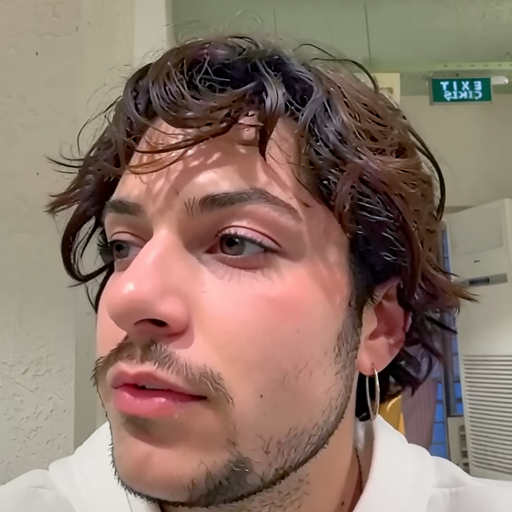
\includegraphics[width=\linewidth]{figures/faceswap_12_raw_head_swap_frame_0175.png}\\[2pt]
    {\scriptsize raw swap}
  \end{minipage}\hspace{0.28cm}%
  \begin{minipage}[b]{3.6cm}
    \centering
    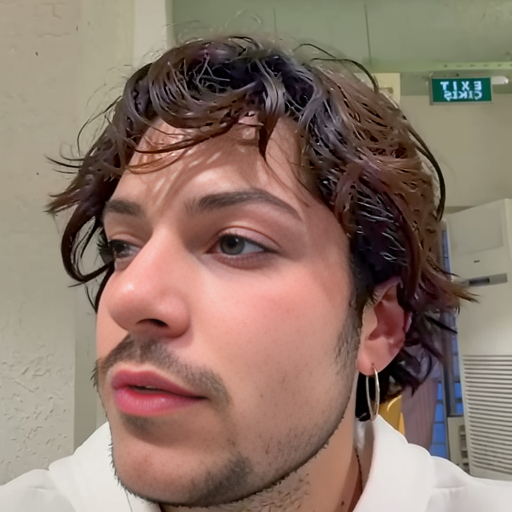
\includegraphics[width=\linewidth]{figures/faceswap_13_restored_frame_0175.png}\\[2pt]
    {\scriptsize after restoration}
  \end{minipage}\hspace{0.28cm}%
  \begin{minipage}[b]{3.6cm}
    \centering
    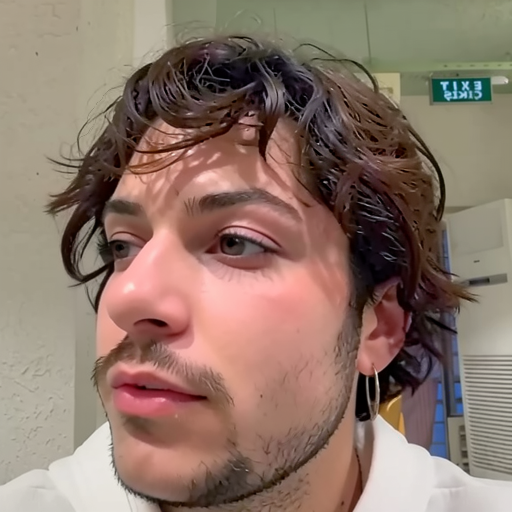
\includegraphics[width=\linewidth]{figures/faceswap_14_smoothed_frame_0175.png}\\[2pt]
    {\scriptsize after smoothing}
  \end{minipage}
  \caption{The same frame 0175 at four points of the flow; the four images are all 512x512.}
  \label{fig:stage_strip}
\end{figure}

\subsection{Problems and decisions}
Attaching the adapter before the first forward pass cost 46 to 48 seconds per frame. Attaching it after one plain pass cost 16 seconds per frame. Peak VRAM was the same in both orders.

We standardised on the fast order. The internal cause was not established, but the effect reproduces exactly and explains an earlier timing discrepancy.

One fixed seed covers the whole clip, so the noise input is constant. The boil still happens, because the model is sensitive to small input changes. Only a pass across frames reduces it.

Memory set the last limit; larger references do not fit. The largest reference we could use is 256 pixels.

\subsection{Limits}
The results table shows a mean at the control level, but the tail stays high, so the picture still jumped on some frames. Each step works inside a frame or a short window, so no step removed that tail. The 256-pixel reference maximum is the second limit on this card.
